\section{Managing the Linux kernel configuration}

\begin{frame}{Kernel version}
  \begin{itemize}
  \item Most packages in Buildroot have a version fixed in their
    corresponding Buildroot package
  \item Some packages are more hardware-related, and there is a need
    to configure their version in a custom way
    \begin{itemize}
    \item Linux kernel, bootloaders, firmware, etc.
    \end{itemize}
  \item Linux kernel version options:
    \begin{itemize}
    \item Latest version
    \item Latest CIP SLTS
    \item Latest CIP RT SLTS
    \item Custom version
    \item Custom Git repository
    \item Custom Mercurial repository
    \item Custom Subversion repository
    \end{itemize}
  \item Using a custom version is recommended $\rightarrow$ ensures
    that upgrading Buildroot doesn't imply a change in the kernel
    version
  \item No relationship between Buildroot version and kernel version
  \end{itemize}
\end{frame}

\begin{frame}{Kernel version configuration}
  \begin{center}
    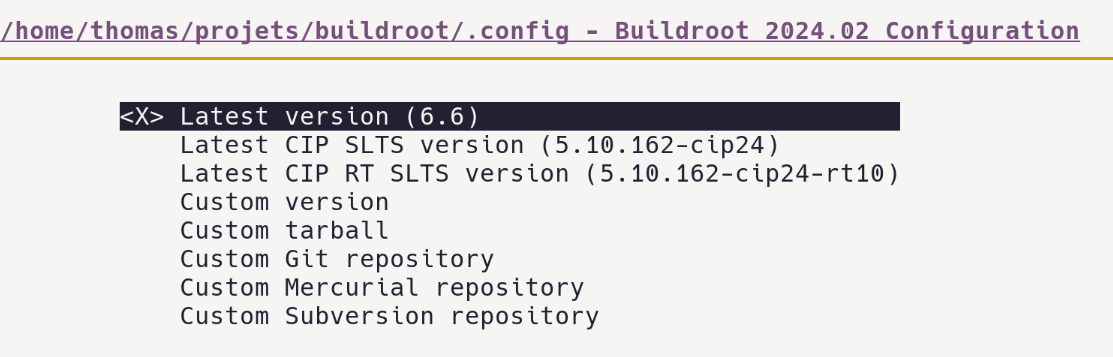
\includegraphics[width=0.8\textwidth]{slides/buildroot-kernel/kernel-version.png}
  \end{center}
\end{frame}

\begin{frame}{Kernel configuration vs. Buildroot configuration}
  \begin{itemize}
  \item The Linux kernel itself uses {\em kconfig} to define its
    configuration
  \item Buildroot cannot replicate all Linux kernel configuration
    options in its \code{menuconfig}
  \item Defining the Linux kernel configuration therefore needs to be
    done in a special way.
  \item Note: while described with the example of the Linux kernel,
    this discussion is also valid for other packages using {\em
      kconfig}: \code{barebox}, \code{uclibc}, \code{busybox} and
    \code{uboot}.
  \end{itemize}
\end{frame}

\begin{frame}{Defining the configuration}
  \begin{itemize}
  \item In the \code{Kernel} menu in \code{menuconfig}, 3
    possibilities to configure the kernel:
    \begin{enumerate}
    \item \code{Use a defconfig}
      \begin{itemize}
      \item Will use a {\em defconfig} provided within the kernel
        sources
      \item Available in \code{arch/<ARCH>/configs} in the kernel
        sources
      \item Used unmodified by Buildroot
      \item Good starting point
      \end{itemize}
    \item \code{Use a custom config file}
      \begin{itemize}
      \item Allows to give the path to either a full \code{.config},
        or a minimal {\em defconfig}
      \item Usually what you will use, so that you can have a custom
        configuration
      \end{itemize}
    \item \code{Use the architecture default configuration}
      \begin{itemize}
      \item Use the {\em defconfig} provided by the architecture in
        the kernel source tree. Some architectures (e.g ARM64) have a
        single {\em defconfig}.
      \end{itemize}
    \end{enumerate}
  \item Configuration can be further tweaked with \code{Additional
      fragments}
    \begin{itemize}
    \item Allows to pass a list of configuration file fragments.
    \item They can complement or override configuration options
      specified in a {\em defconfig} or a full configuration file.
    \end{itemize}
  \end{itemize}
\end{frame}

\begin{frame}[fragile]{Examples of kernel configuration}

  \scriptsize

  \begin{block}{{\tt stm32mp157a\_dk1\_defconfig}: custom configuration file}
\begin{verbatim}
BR2_LINUX_KERNEL_USE_CUSTOM_CONFIG=y
BR2_LINUX_KERNEL_CUSTOM_CONFIG_FILE="board/stmicroelectronics/stm32mp157a-dk1/linux.config"
\end{verbatim}
  \end{block}

  \begin{block}{{\tt ts4900\_defconfig}: standard kernel defconfig}
\begin{verbatim}
BR2_LINUX_KERNEL_DEFCONFIG="imx_v6_v7"
\end{verbatim}
  \end{block}

  \begin{block}{{\tt warpboard\_defconfig}: standard kernel defconfig + fragment}
\begin{verbatim}
BR2_LINUX_KERNEL_DEFCONFIG="imx_v6_v7"
BR2_LINUX_KERNEL_CONFIG_FRAGMENT_FILES="board/freescale/warpboard/linux.fragment"
\end{verbatim}
  \end{block}

  \begin{block}{{\tt linux.fragment}: contains extra kernel options}
\begin{verbatim}
CONFIG_CFG80211_WEXT=y
\end{verbatim}
  \end{block}

\end{frame}

\begin{frame}{Changing the configuration}
  \begin{itemize}
  \item Running one of the Linux kernel configuration interfaces:
    \begin{itemize}
    \item \code{make linux-menuconfig}
    \item \code{make linux-nconfig}
    \item \code{make linux-xconfig}
    \item \code{make linux-gconfig}
    \end{itemize}
  \item Will load either the defined kernel {\em defconfig} or custom
    configuration file, and start the corresponding Linux kernel
    configuration interface.
  \item Changes made are only made in
    \code{$(O)/build/linux-<version>/}, i.e. they are not preserved
    across a clean rebuild.
  \item To save them:
    \begin{itemize}
    \item \code{make linux-update-config}, to save a full config file
    \item \code{make linux-update-defconfig}, to save a minimal
      defconfig
    \item Only works if a {\em custom configuration file} is used
    \end{itemize}
  \end{itemize}
\end{frame}

\begin{frame}{Typical flow}
  \begin{enumerate}
  \item \code{make menuconfig}
    \begin{itemize}
    \item Start with a {\em defconfig} from the kernel, say \code{mvebu_v7_defconfig}
    \end{itemize}
  \item Run \code{make linux-menuconfig} to customize the
    configuration
  \item Do the build, test, tweak the configuration as needed.
  \item You cannot do \code{make linux-update-{config,defconfig}},
    since the Buildroot configuration points to a kernel {\em
      defconfig}
  \item \code{make menuconfig}
    \begin{itemize}
    \item Change to a custom configuration file. There's no need for
      the file to exist, it will be created by Buildroot.
    \end{itemize}
  \item \code{make linux-update-defconfig}
    \begin{itemize}
    \item Will create your custom configuration file, as a minimal
      {\em defconfig}
    \end{itemize}
  \end{enumerate}
\end{frame}
